% VISUAL-FIRST REVIEW POSTER (2026-10-19). For collaborator review (Toni, Chris, Pierce); NOT for print until approved.
% The submitted poster docs/summit_poster/poster.pdf is unchanged.
% Numbers: records/CORA_SUMMIT_CLAIM_LEDGER_20261017.md (audited in POSTER_CLAIM_AUDIT.md).
% Figures: figures/ (drawn by scripts/summit_visual_figures.py from hash-pinned recorded inputs; provenance in
% POSTER_FIGURE_PROVENANCE.json). The one illustrative figure says so on its face.
% Diagrams: TikZ. Solid outline = implemented and tested; dashed = proposed or not yet validated.
% Size: A0 portrait is a REVIEW ASSUMPTION (no organizer guide on file). Body 30 pt; figure text >= 20 pt.
% Build: see REVIEW_CHECKLIST.md (fixed SOURCE_DATE_EPOCH, no trailer id).
\RequirePackage{fix-cm}
\documentclass[25pt, a0paper, portrait, blockverticalspace=7mm]{tikzposter}
\usepackage[scaled]{helvet}
\renewcommand{\familydefault}{\sfdefault}
\usepackage[T1]{fontenc}
\usepackage{graphicx}
\usepackage{enumitem}
\usepackage{array}
\usetikzlibrary{positioning, arrows.meta, fit, calc, shapes.geometric}
\pdftrailerid{}

\newcommand{\bodyfont}{\fontsize{30}{38}\selectfont\raggedright}
\newcommand{\secfont}{\fontsize{26}{32}\selectfont\raggedright}
\newcommand{\diagfont}{\fontsize{26}{31}\selectfont}
\newcommand{\diagsub}{\fontsize{22}{27}\selectfont}
\newcommand{\bignum}[1]{{\fontsize{120}{120}\selectfont\bfseries #1}}
\newcommand{\bt}[1]{{\fontsize{40}{48}\selectfont #1}}
\newcommand{\chip}[2]{{\fontsize{26}{30}\selectfont\color{#1}\,[#2]}}
\setlist{leftmargin=1.1em, itemsep=0.2em, topsep=0.2em, parsep=0pt}

\definecolor{ink}{HTML}{0B0B0B}
\definecolor{ink2}{HTML}{52514E}
\definecolor{accent}{HTML}{2A78D6}
\definecolor{warm}{HTML}{EB6834}
\definecolor{good}{HTML}{0CA30C}
\definecolor{neutral}{HTML}{F0EFEC}
\definecolor{critical}{HTML}{D03B3B}
\definecolor{paper}{HTML}{FCFCFB}
\definecolor{arcblue}{HTML}{0074D9}
\definecolor{arcred}{HTML}{FF4136}

\usetheme{Simple}
\tikzposterlatexaffectionproofoff
\colorlet{backgroundcolor}{paper}
\colorlet{framecolor}{paper}
\colorlet{titlefgcolor}{ink}
\colorlet{titlebgcolor}{paper}
\colorlet{blocktitlebgcolor}{paper}
\colorlet{blocktitlefgcolor}{accent}
\colorlet{blockbodybgcolor}{paper}
\colorlet{blockbodyfgcolor}{ink}
\makeatletter
\settitle{\centering\vbox{\color{titlefgcolor}{\bfseries\fontsize{100}{112}\selectfont \@title\par}\vspace*{0.2em}%
  {\fontsize{52}{62}\selectfont \@author\par}\vspace*{0.25em}{\fontsize{36}{44}\selectfont\color{ink2} \@institute}}}
\makeatother

\title{LEARNING WHAT TO CHANGE}
\author{From Visual Reasoning to Scientific Hypothesis Revision}
\institute{Chimdi Walter Ndubuisi \,$\cdot$\, University of Missouri \quad {\color{critical}REVIEW DRAFT 19 October: for collaborator review, not for print}}

\tikzset{
  stage/.style={rounded corners=8pt, draw=accent, line width=2.6pt, fill=white, align=center, font=\diagfont,
                inner sep=9pt},
  pstage/.style={stage, dashed, draw=ink2, dash pattern=on 12pt off 7pt},
  test/.style={stage, draw=ink, line width=3.4pt, fill=neutral},
  flow/.style={-{Latex[length=8mm,width=6mm]}, line width=2.8pt, draw=ink2},
  lab/.style={font=\diagsub, text=ink2, align=center},
}

\begin{document}
\maketitle[width=0.97\linewidth]

%======================= THE CENTRAL QUESTION (full width)
\block{}{%
  \centering
  {\fontsize{58}{68}\selectfont\bfseries Can a reasoner recognize when its explanation is inadequate,\\[0.1em]
   and determine what needs to change?\par}
  \vspace{0.35em}
  {\fontsize{30}{37}\selectfont\color{ink2} Solving a problem is not the same as knowing why the solution works, or what
   to change when the available concepts and rules fall short. A question shaped in discussions with Toni Kazic.\par}
  \vspace{0.25em}
  {\fontsize{30}{37}\selectfont \textbf{Aims}, not yet all achieved: find objects and relations $\rightarrow$ write
   executable hypotheses $\rightarrow$ notice inadequacy $\rightarrow$ choose a justified revision $\rightarrow$ test it
   independently $\rightarrow$ transfer the procedure.\par}
}

\begin{columns}

%======================= COLUMN 1: the big question, and why ARC is a useful test
\column{0.333}
\block{\bt{1 \;$\cdot$\; Why ARC is a useful test}}{\bodyfont
  ARC tasks require inferring a transformation from a few examples and applying it to a new input.
  \begin{tikzfigure}
    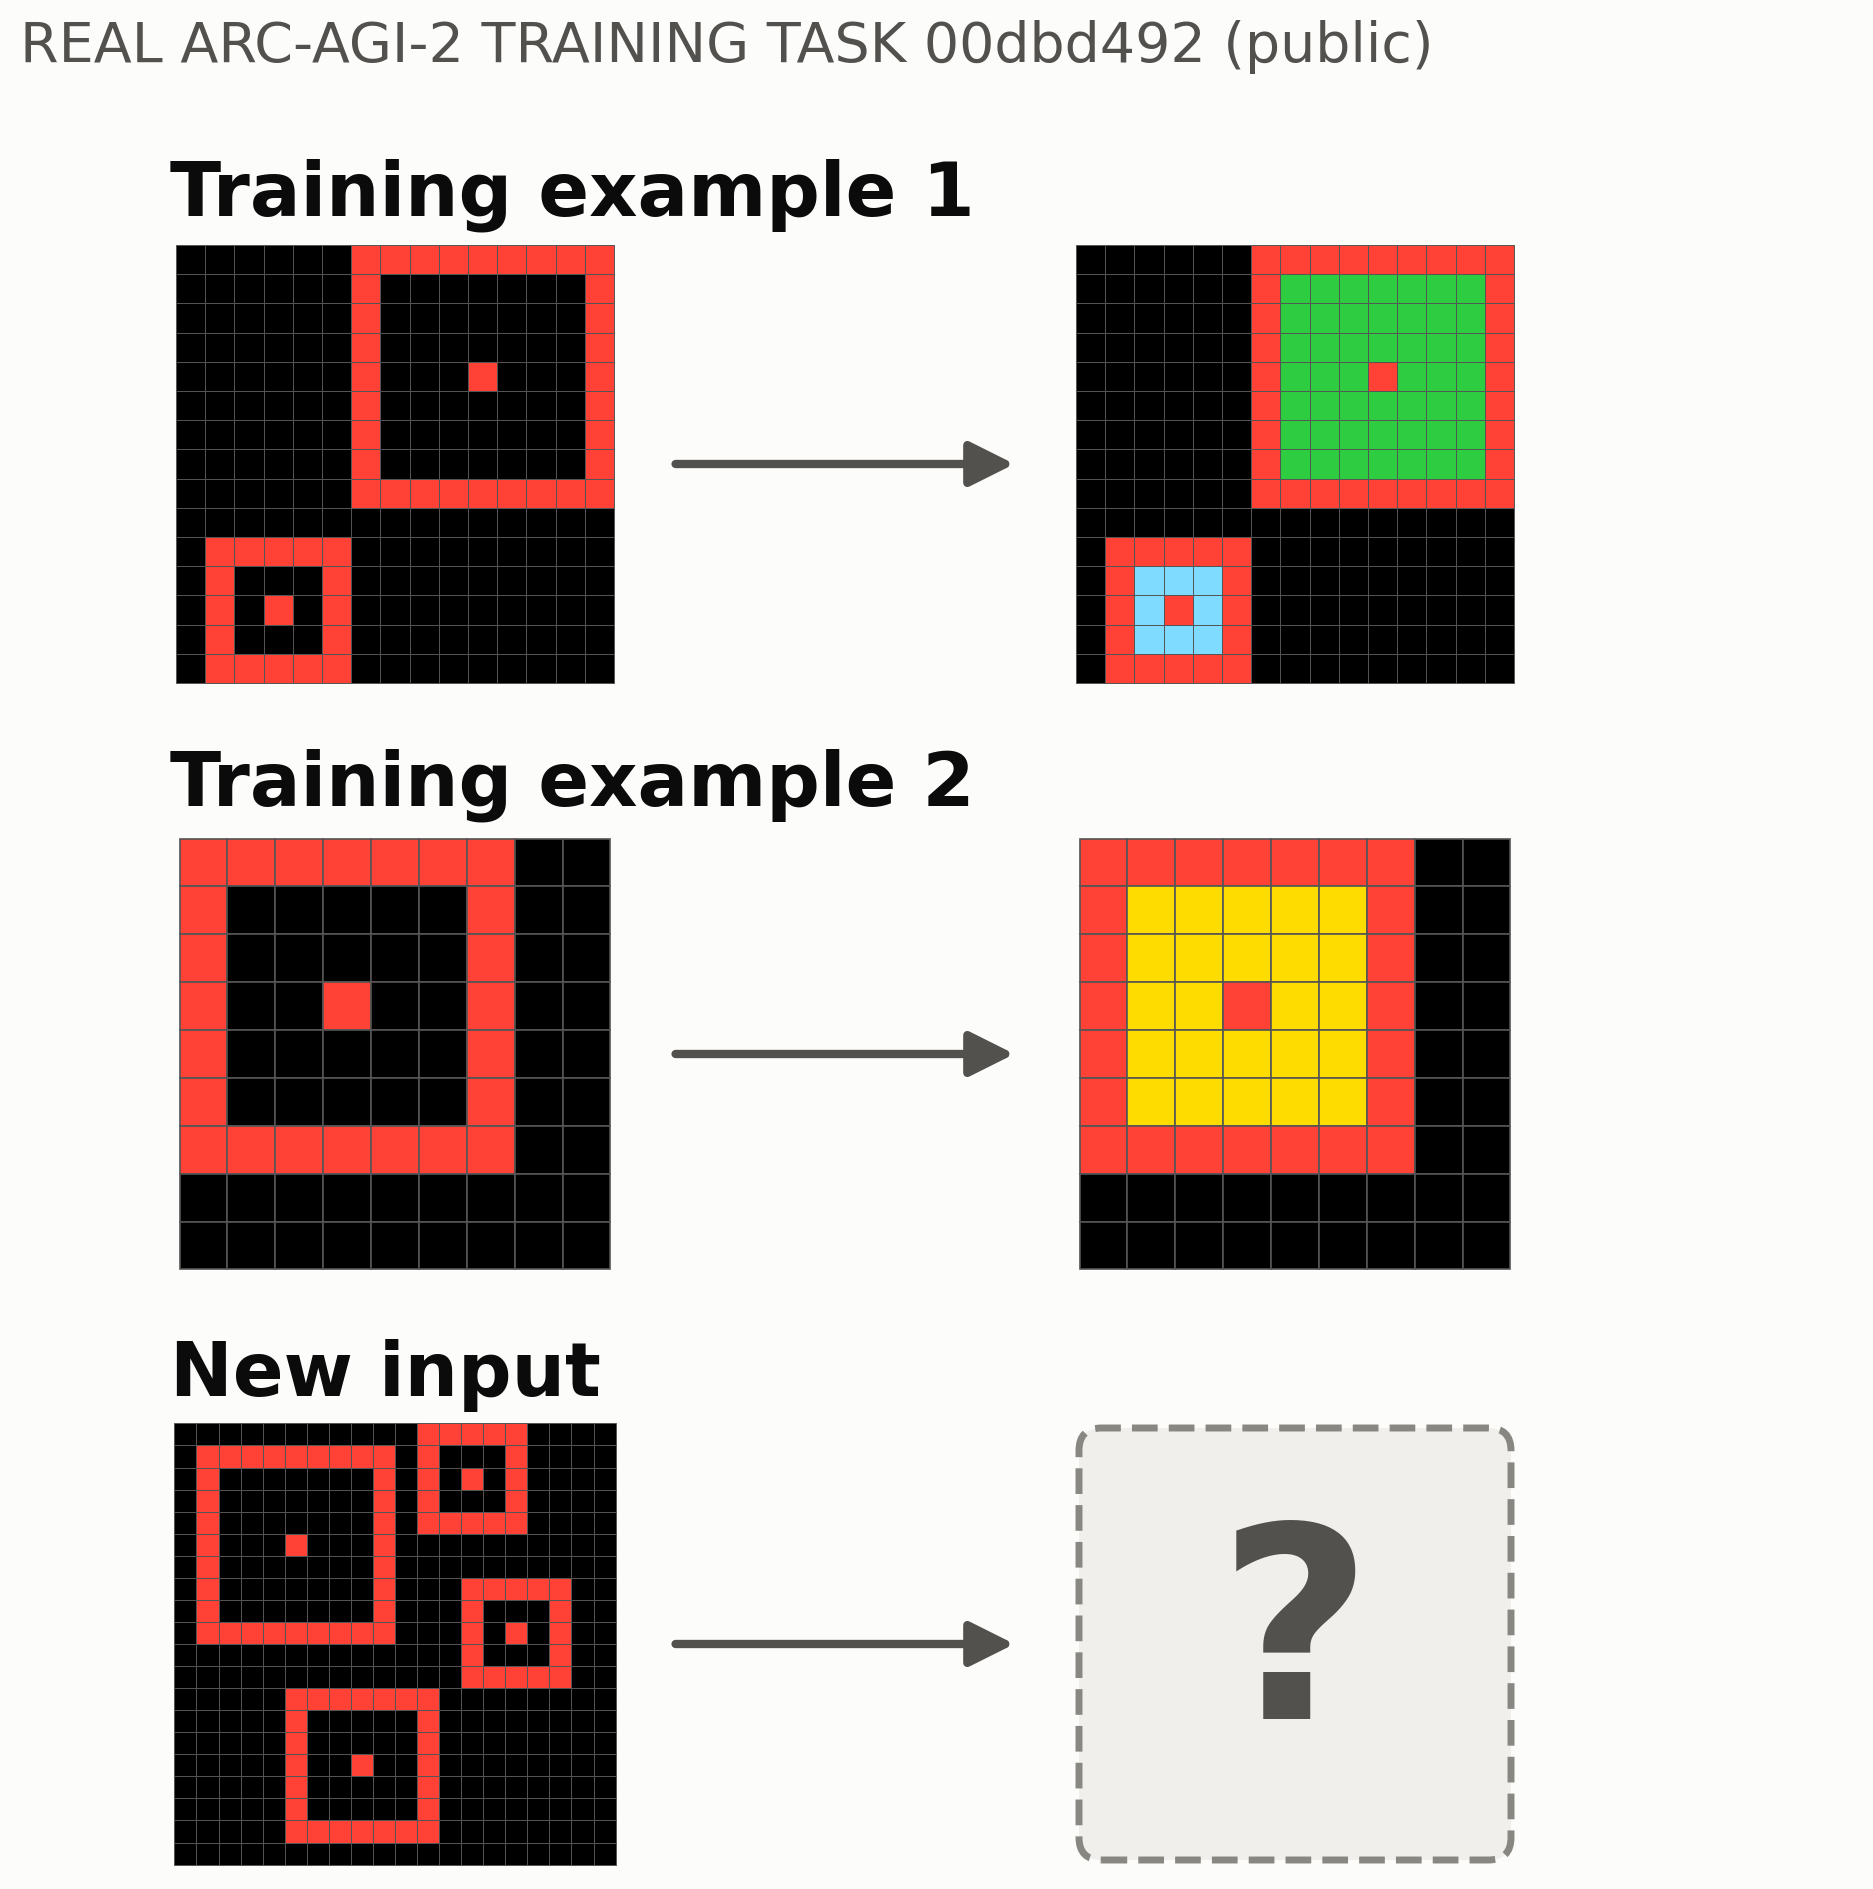
\includegraphics[width=\linewidth]{figures/fig_arc_intro_00dbd492.png}
  \end{tikzfigure}
  \secfont\color{ink2} Each frame's fill colour depends on its size.
}
\block{\bt{Four reasons to revise}}{\bodyfont
  \begin{tikzfigure}
    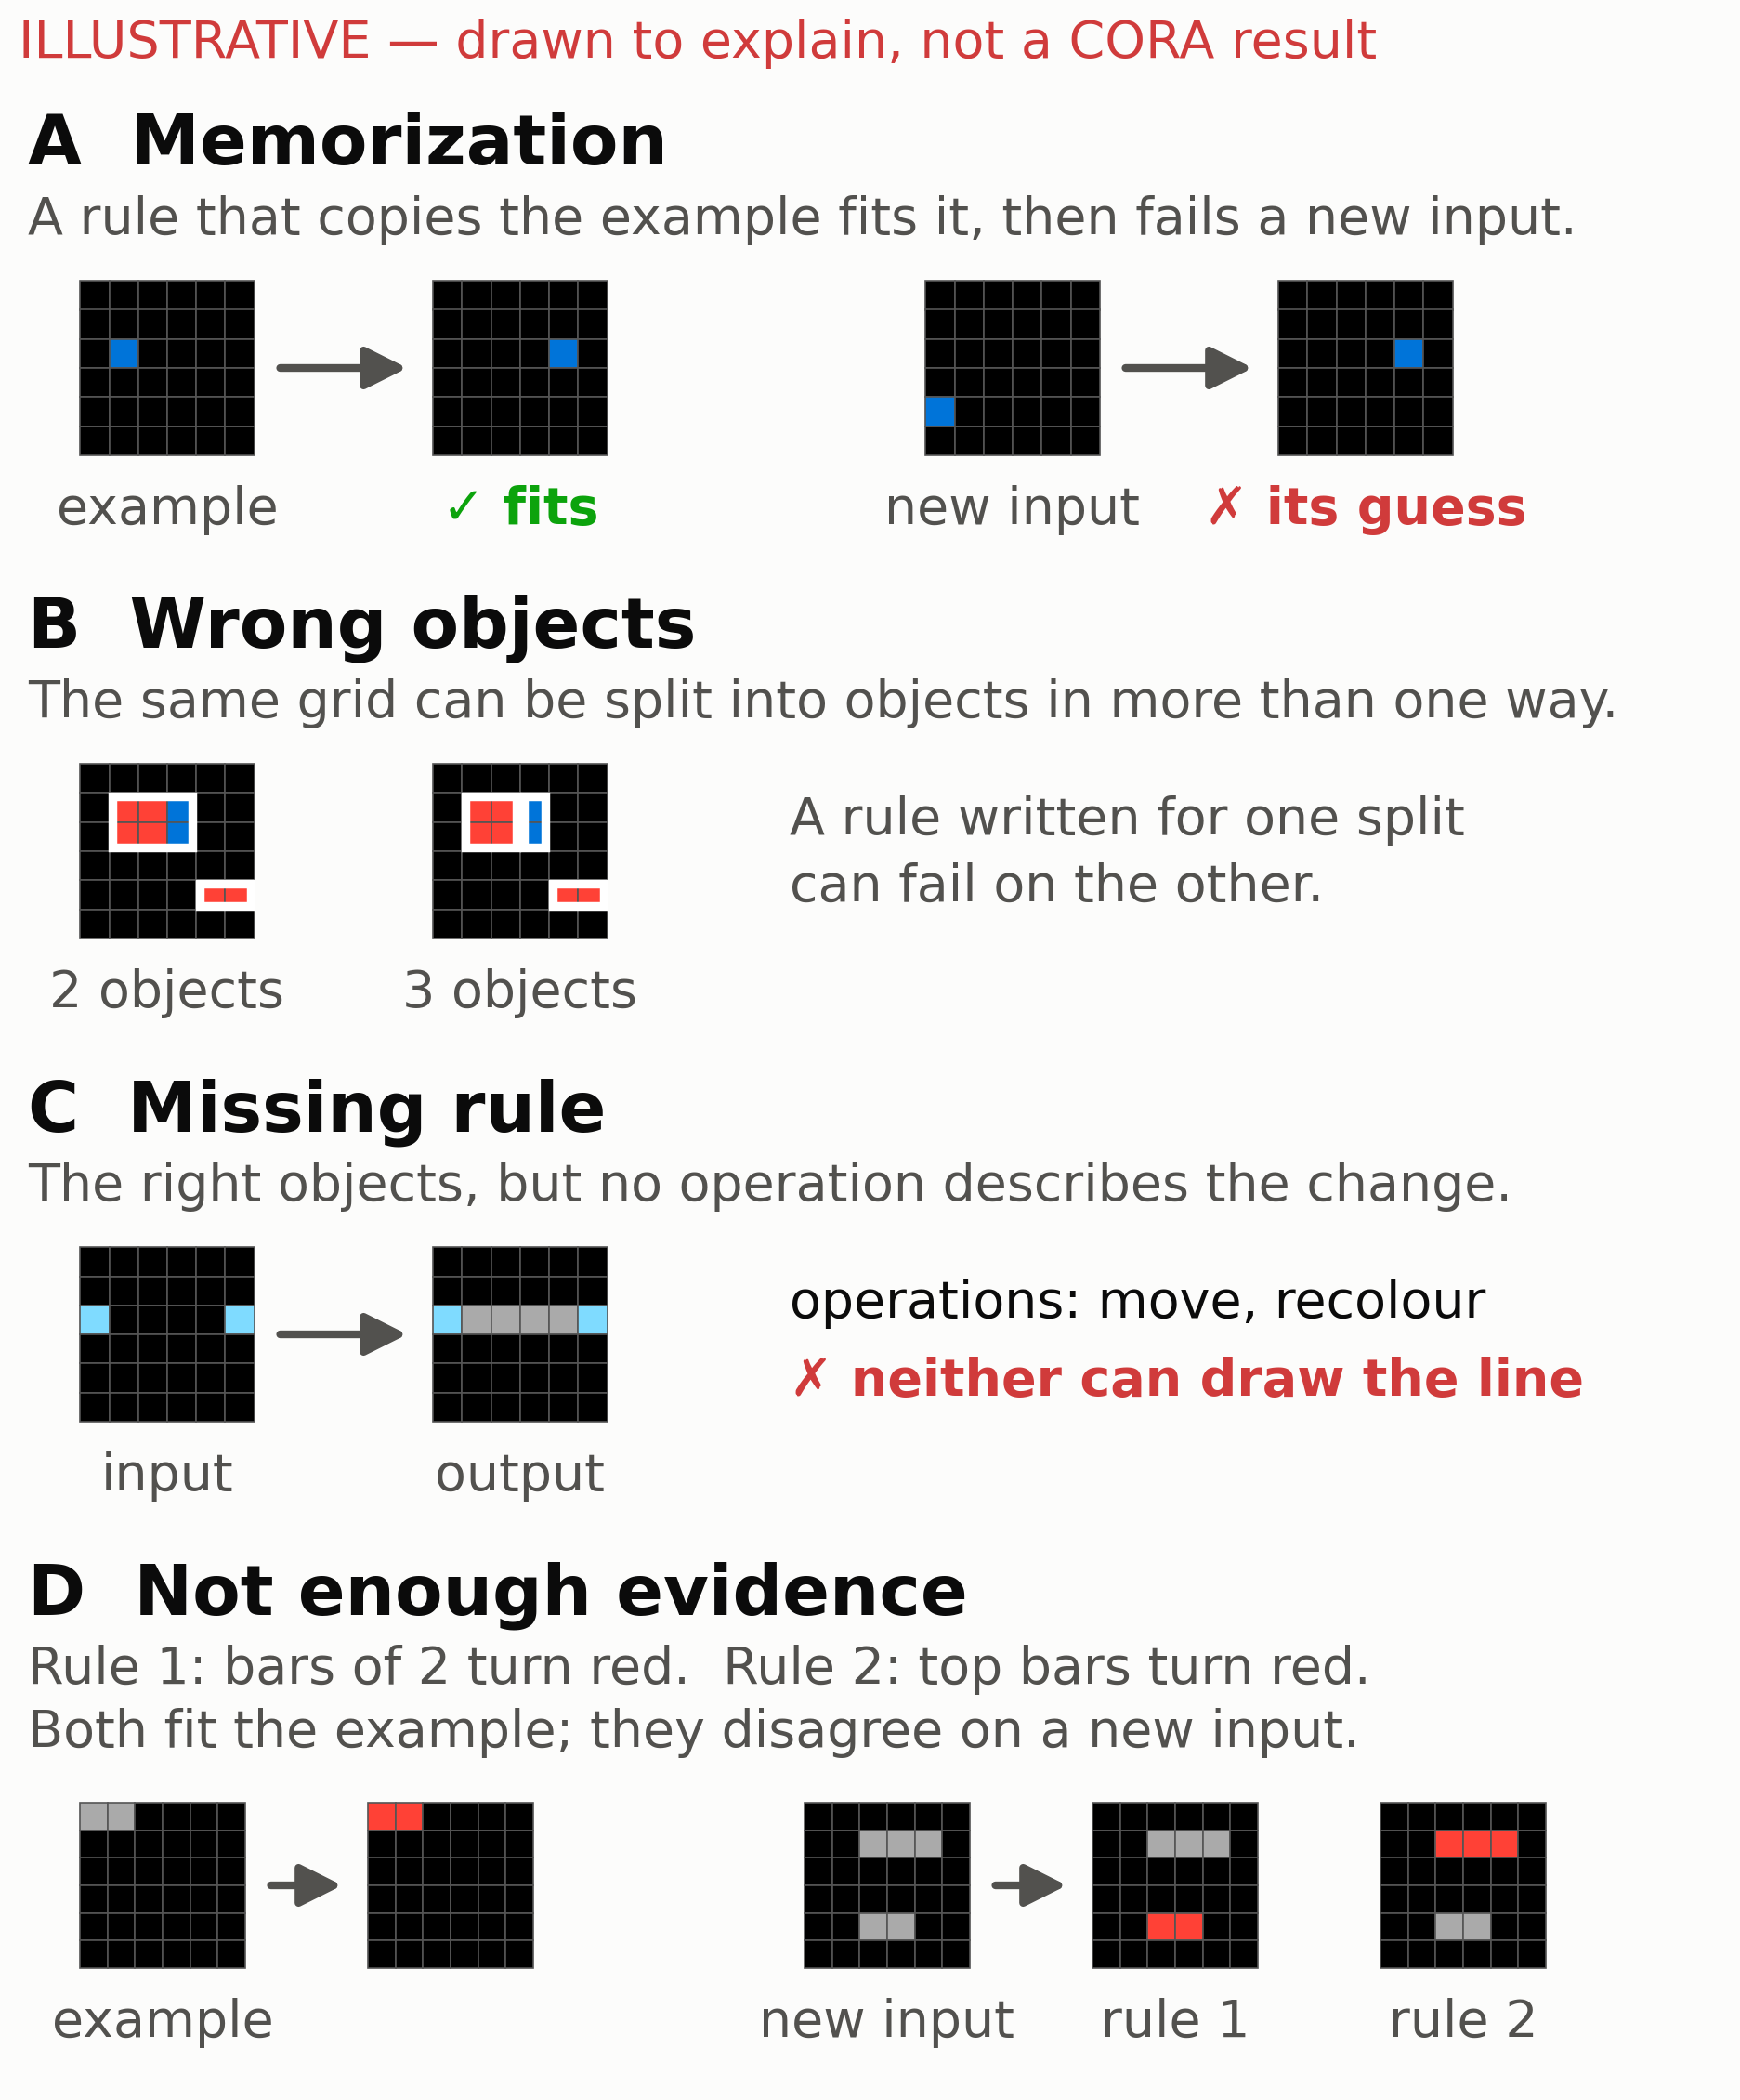
\includegraphics[width=\linewidth]{figures/fig_four_reasons_ILLUSTRATIVE.png}
  \end{tikzfigure}
  These are different possible causes. Telling them apart, from the examples alone, is the research problem.
}

%======================= COLUMN 2: CORA, what I built, tested and discovered
\column{0.333}
\block{\bt{2 \;$\cdot$\; CORA: what I built}}{\bodyfont
  CORA is an executable ARC reasoning system used to investigate how models construct, test and revise hypotheses
  from sparse visual examples.
  \begin{tikzfigure}
  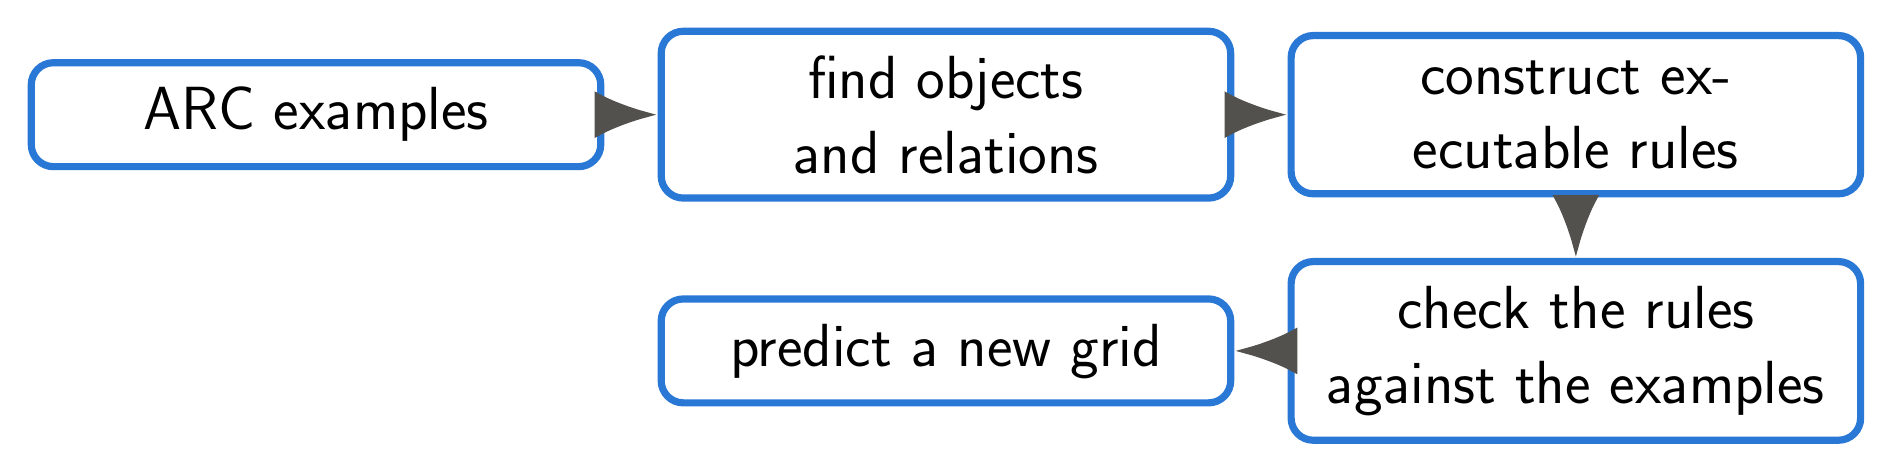
\begin{tikzpicture}
    \node[stage, text width=6.6cm, font=\diagsub] (a) at (0,0) {ARC examples};
    \node[stage, text width=6.6cm, font=\diagsub] (b) at (8,0) {find objects and relations};
    \node[stage, text width=6.6cm, font=\diagsub] (c) at (16,0) {construct executable rules};
    \node[stage, text width=6.6cm, font=\diagsub] (d) at (16,-3.0) {check the rules against the examples};
    \node[stage, text width=6.6cm, font=\diagsub] (e) at (8,-3.0) {predict a new grid};
    \draw[flow] (a) -- (b); \draw[flow] (b) -- (c); \draw[flow] (c) -- (d); \draw[flow] (d) -- (e);
  \end{tikzpicture}
  \end{tikzfigure}
}
\block{\bt{Fitting is not enough}\chip{good}{DONE}}{\bodyfont
  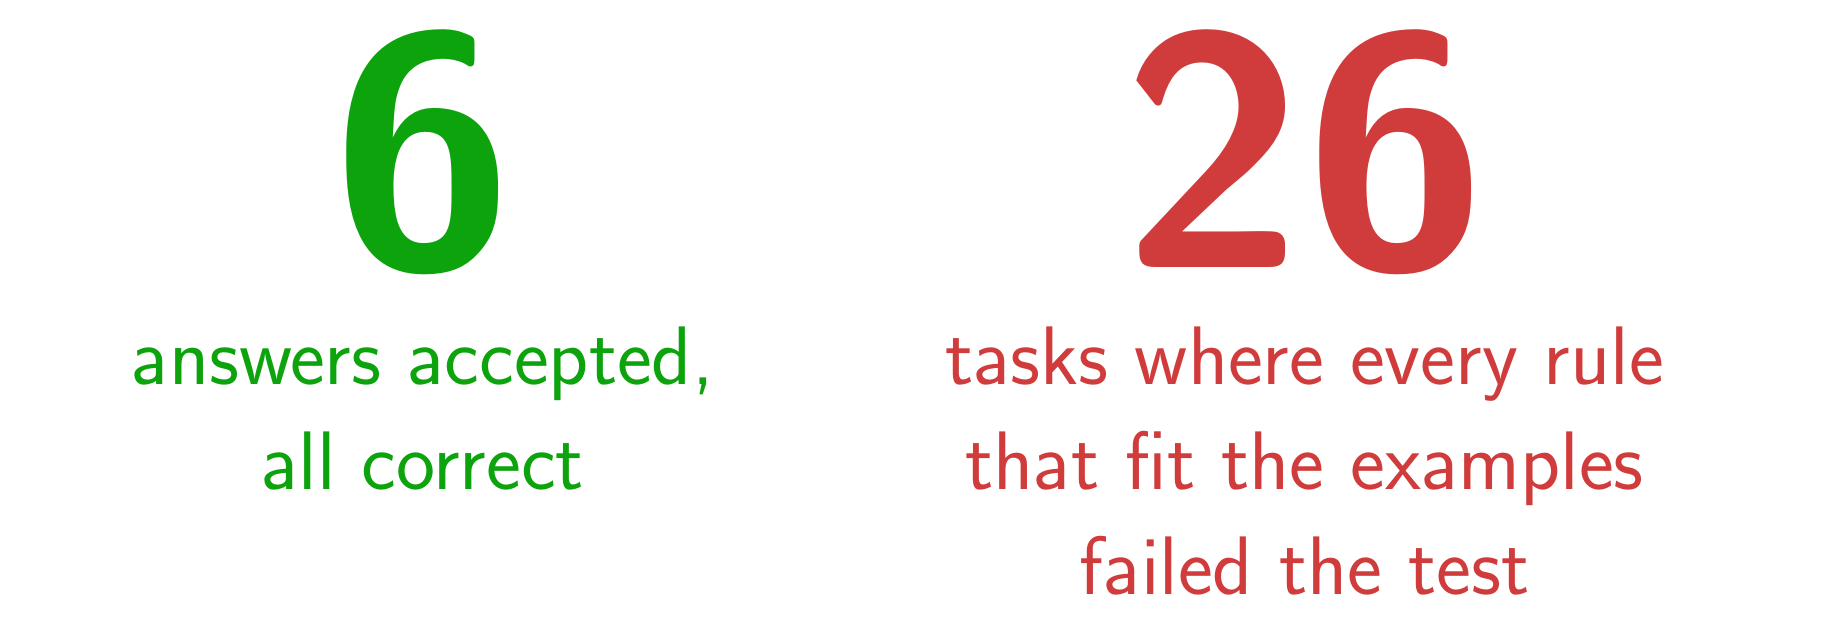
\begin{tikzpicture}
    \node[anchor=north, text width=9.8cm, align=center, font=\fontsize{30}{38}\selectfont] at (0,0)
      {\color{good}\bignum{6}\\[0.15em] answers accepted,\\ all correct};
    \node[anchor=north, text width=12.2cm, align=center, font=\fontsize{30}{38}\selectfont] at (11.2,0)
      {\color{critical}\bignum{26}\\[0.15em] tasks where every rule\\ that fit the examples\\ failed the test};
  \end{tikzpicture}
  \par\secfont\color{ink2} 60 exposed ARC-AGI-2 training tasks; CORA's object reasoner as submitted.
}
\block{\bt{A rule CORA built}\chip{good}{DONE, NARROW}}{\bodyfont
  \begin{tikzfigure}
    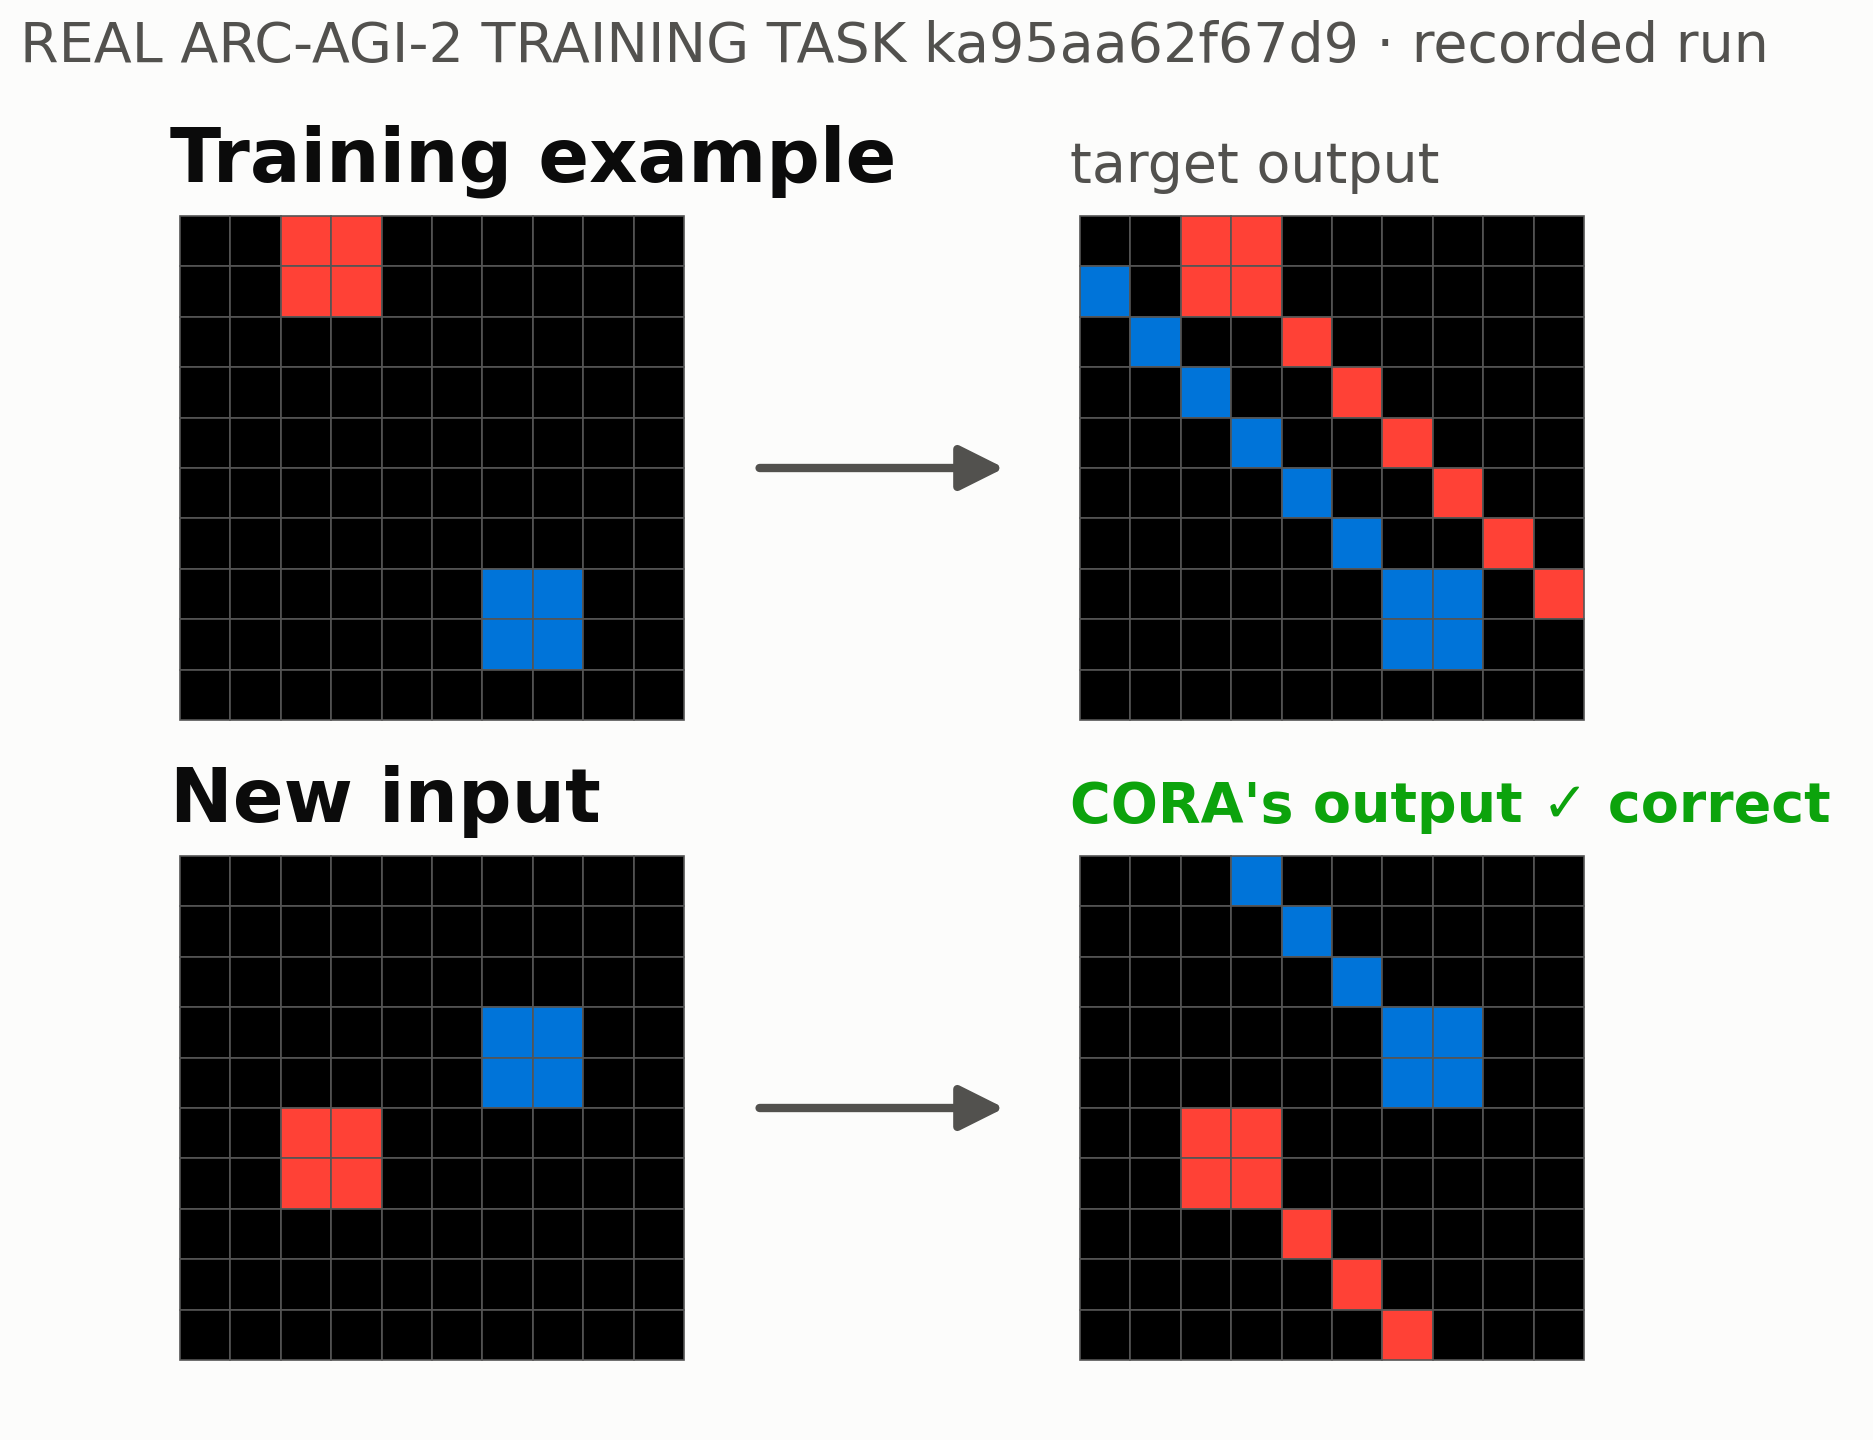
\includegraphics[width=\linewidth]{figures/fig_real_rule_ka95aa62f67d9.png}
  \end{tikzfigure}
  Depending on an object's colour, extend a line toward one of two corners:
  {\color{arcblue}\textbf{blue}} up-left, {\color{arcred}\textbf{red}} down-right.
  \par\vspace{0.25em}\secfont
  Automatically constructed conditional operation; rebuilt 3 of 3 times with one example held out.
  {\color{ink2} An exposed task chosen in development; a constructor that ignored the failure record found the same
  rule, so diagnosis did not cause this gain.}
}
\block{\bt{Did it generalize?}\chip{critical}{NEGATIVE}}{\bodyfont
  \centering{\color{critical}\bignum{0 / 58}}\par\vspace{0.15em}
  new verified solves from rule construction\par\vspace{0.25em}
  \raggedright\secfont\color{ink2} 58 separately selected, still exposed training tasks; every construction variant;
  no wrong answers; no advantage from the failure record.
}
%======================= COLUMN 3: learning what to revise, the next scientific step
\column{0.333}
\block{\bt{3 \;$\cdot$\; Learning what to revise}}{\bodyfont
  \begin{tikzfigure}
  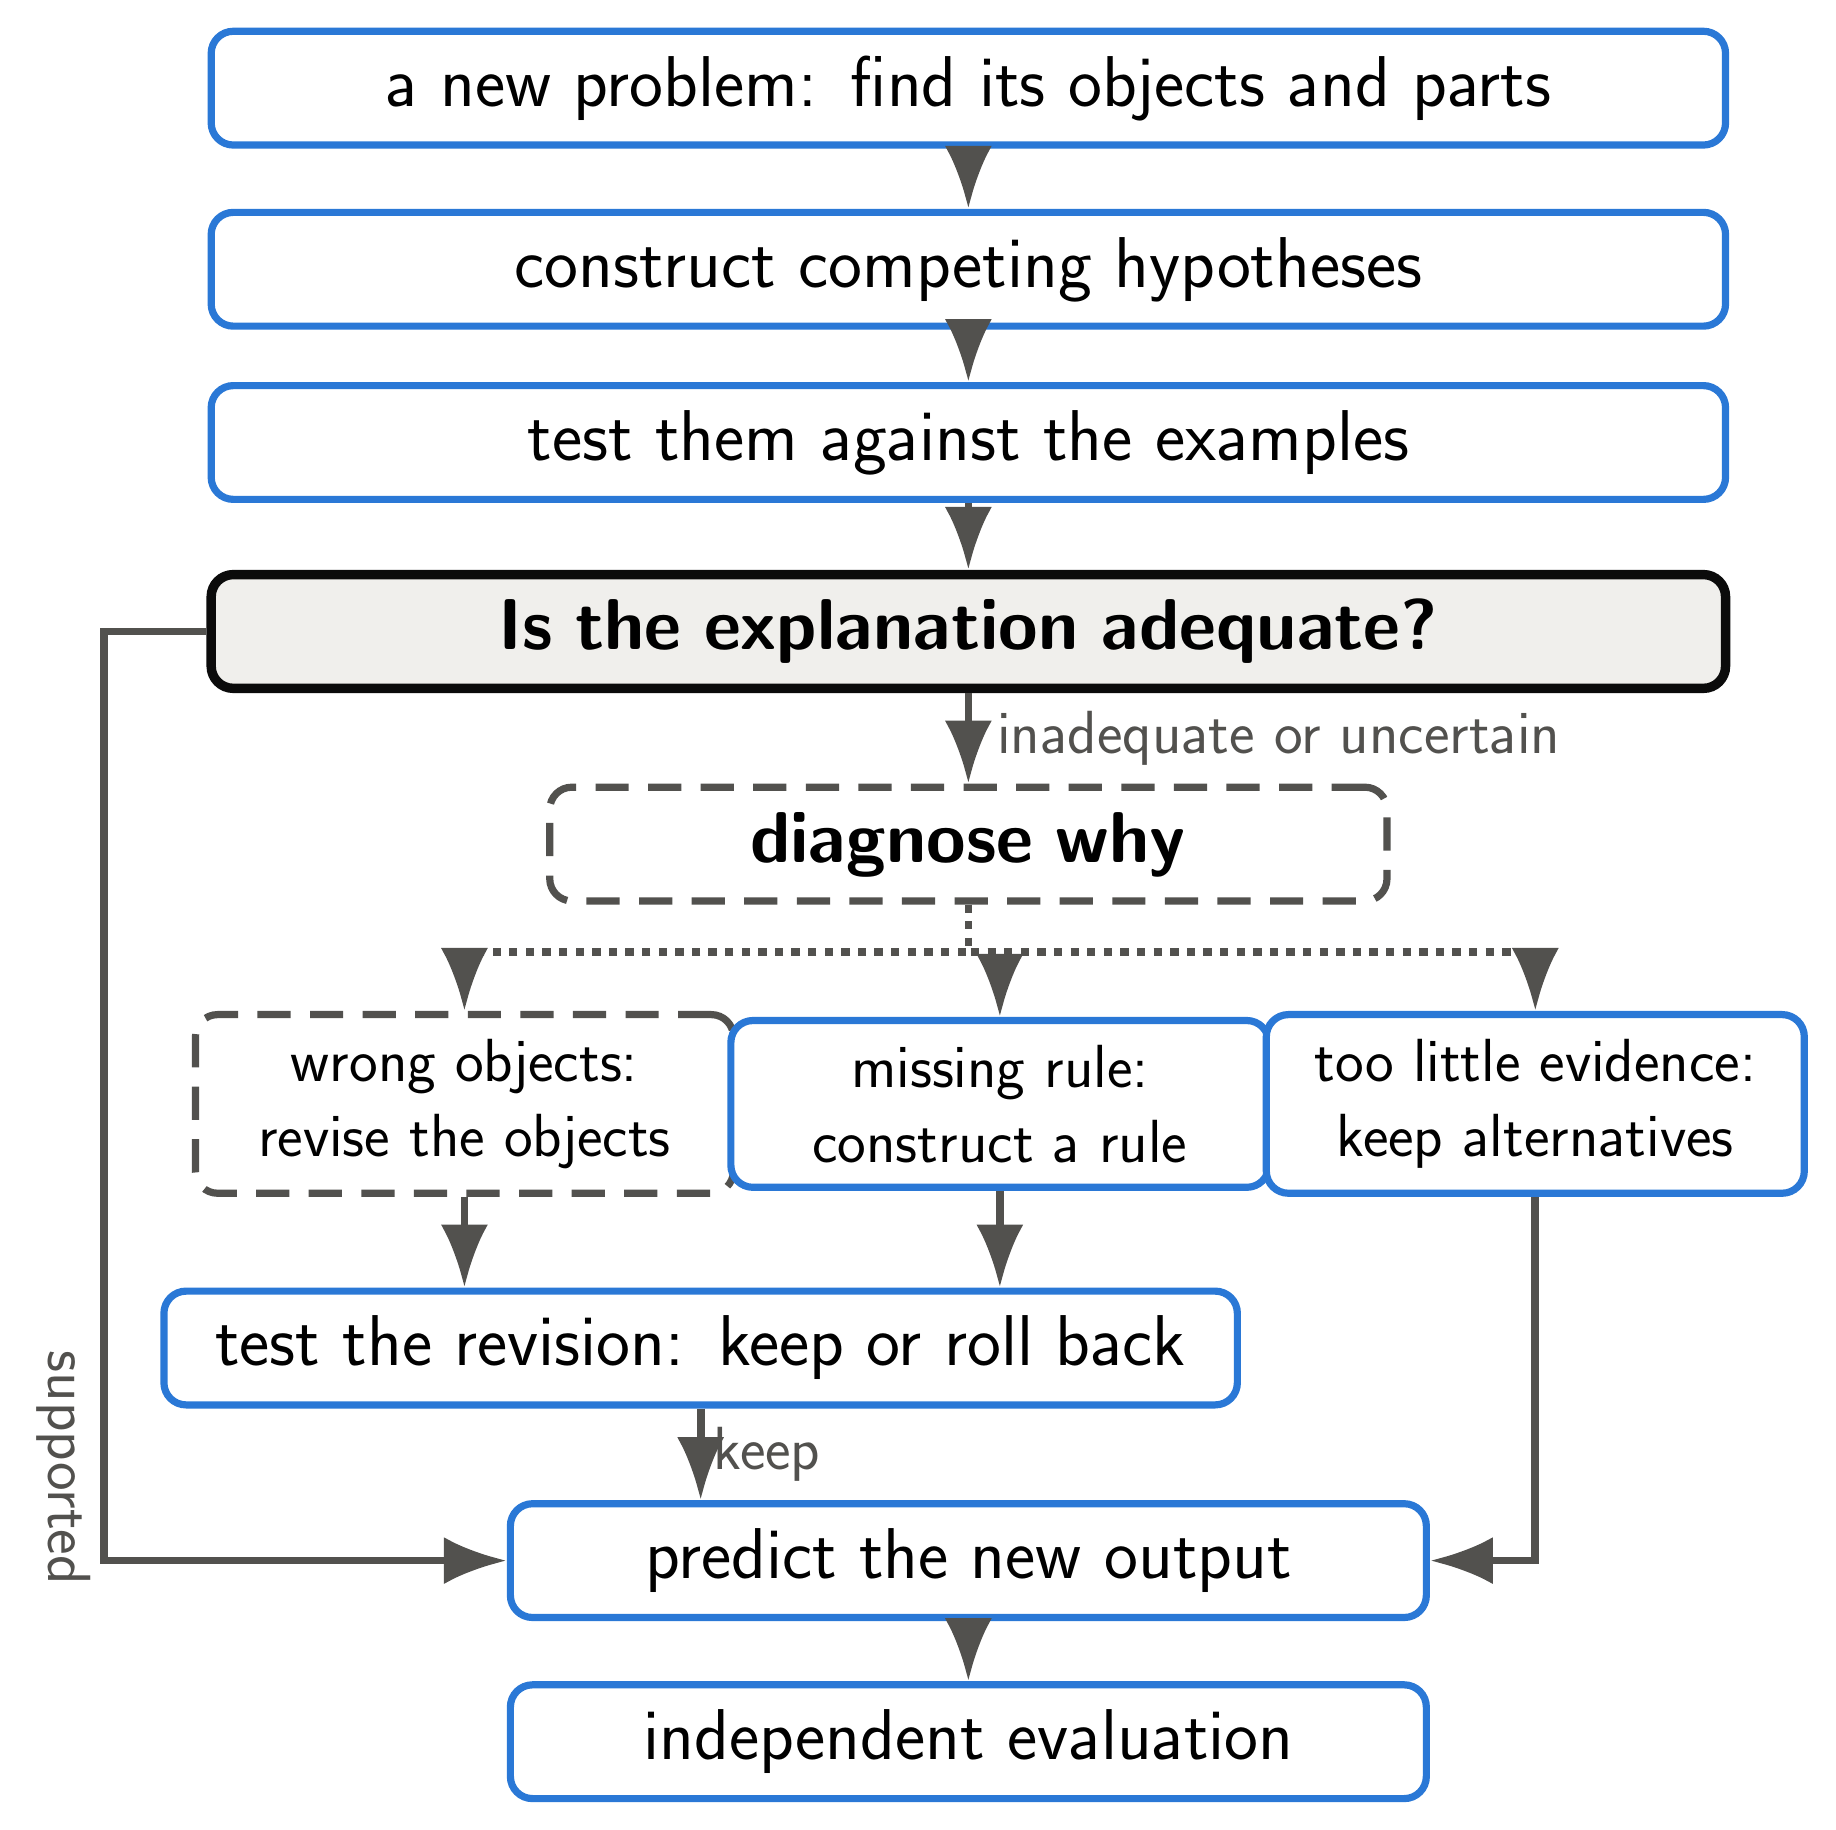
\begin{tikzpicture}
    \node[stage, text width=18.6cm] (i) at (1,0) {a new problem: find its objects and parts};
    \node[stage, text width=18.6cm] (h) at (1,-2.3) {construct competing hypotheses};
    \node[stage, text width=18.6cm] (t) at (1,-4.5) {test them against the examples};
    \node[test, text width=18.6cm] (q) at (1,-6.9) {\textbf{Is the explanation adequate?}};
    \node[pstage, text width=10cm] (dg) at (1,-9.6) {\textbf{diagnose why}};
    \node[pstage, text width=6.2cm, font=\diagsub] (r1) at (-5.4,-12.9) {wrong objects:\\ revise the objects};
    \node[stage, text width=6.2cm, font=\diagsub] (r2) at (1.4,-12.9) {missing rule:\\ construct a rule};
    \node[stage, text width=6.2cm, font=\diagsub] (r3) at (8.2,-12.9) {too little evidence:\\ keep alternatives};
    \node[stage, text width=13cm] (tr) at (-2.4,-16.0) {test the revision: keep or roll back};
    \node[stage, text width=11cm] (pr) at (1,-18.7) {predict the new output};
    \node[stage, text width=11cm] (ev) at (1,-21.0) {independent evaluation};
    \draw[flow] (i) -- (h); \draw[flow] (h) -- (t); \draw[flow] (t) -- (q);
    \draw[flow] (q) -- node[lab, right, xshift=0.2cm] {inadequate or uncertain} (dg);
    \draw[flow, dashed] (dg.south) -- ++(0,-0.6) -| (r1.north);
    \draw[flow, dashed] (dg.south) -- ++(0,-0.6) -| (r2.north);
    \draw[flow, dashed] (dg.south) -- ++(0,-0.6) -| (r3.north);
    \draw[flow] (r1.south) -- (r1.south |- tr.north);
    \draw[flow] (r2.south) -- (r2.south |- tr.north);
    \draw[flow] (r3.south) |- (pr.east);
    \draw[flow] (tr.south) -- node[lab, right] {keep} (tr.south |- pr.north);
    \draw[flow] (q.west) -- ++(-1.3,0) |- node[lab, pos=0.45, below, sloped] {supported} (pr.west);
    \draw[flow] (pr) -- (ev);
  \end{tikzpicture}
  \end{tikzfigure}
  \secfont
  \textbf{Recognizing} an inadequate explanation: partly built (CORA-v2). \textbf{Knowing which revision helps}:
  not yet shown. {\color{ink2} CORA never sees the hidden answer.}
}
\block{\bt{CORA-v2}\chip{warm}{DEVELOPMENT}}{\bodyfont
  Compares alternative executable hypotheses and records why it is uncertain.
  \begin{tikzfigure}
    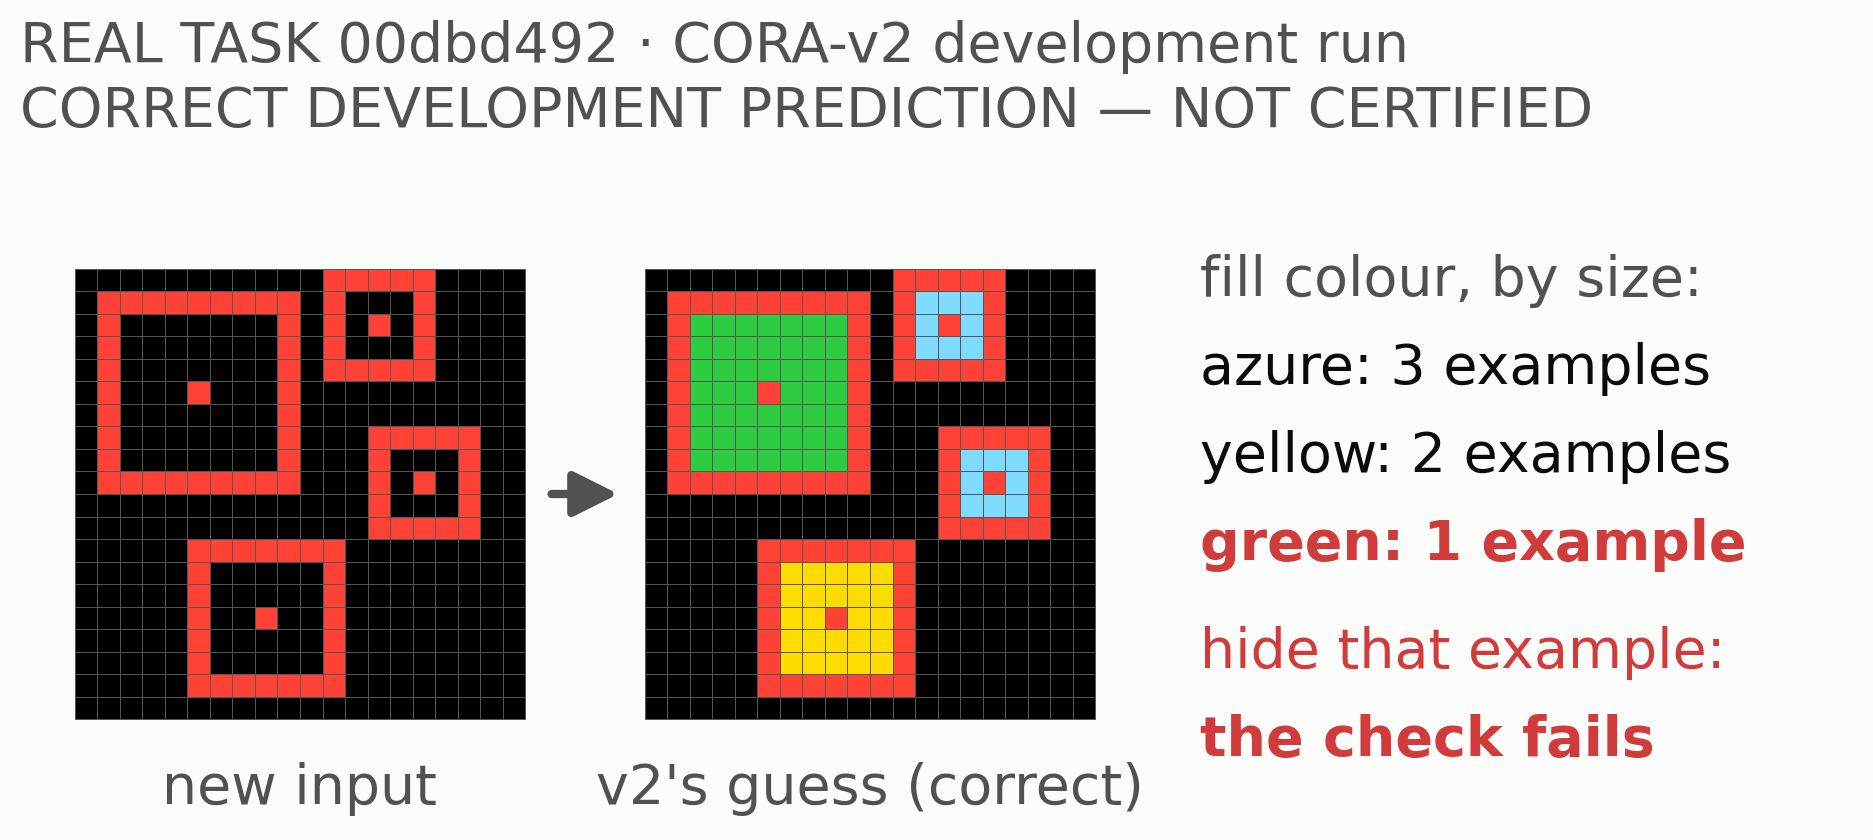
\includegraphics[width=\linewidth]{figures/fig_v2_uncertified_00dbd492_poster.png}
  \end{tikzfigure}
  \secfont\color{ink2} On 118 exposed development tasks: 4 correct and 1 wrong exploratory guesses; nothing certified.
}
\block{\bt{Inventing new operations}\chip{ink2}{RUNNING}}{\secfont
  \textbf{Automatic rule-language extension}, a separate CORA experiment: can a system build new reusable
  operations itself? 475 of 497 proposal units done (19 October); no verdict; not part of CORA-v2 or any Kaggle
  entry.
}
\block{\bt{From ARC to science}\chip{critical}{FUTURE, NOT TESTED}}{\secfont
  \begin{tikzfigure}
  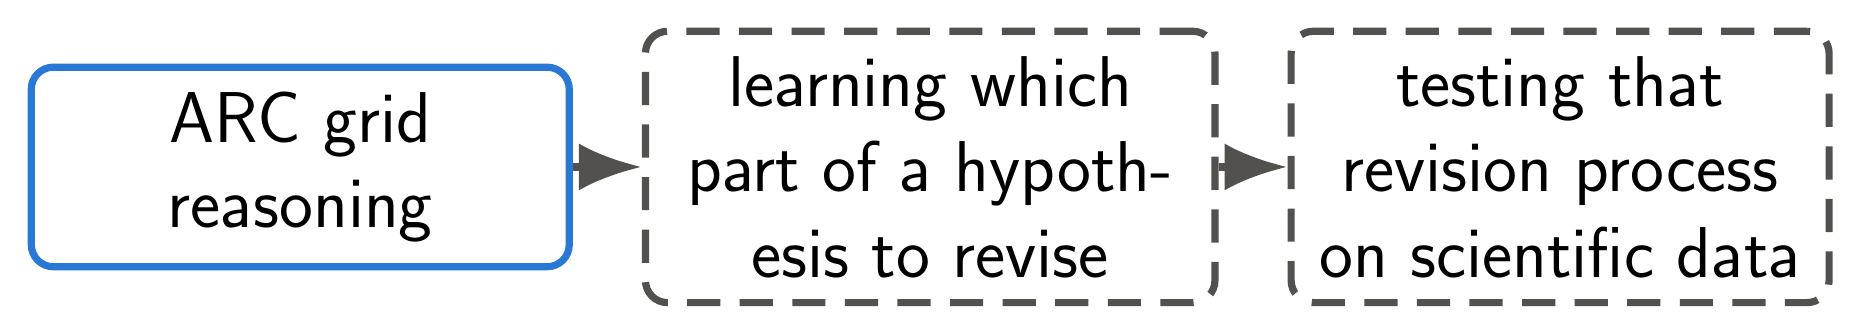
\begin{tikzpicture}
    \node[stage, text width=6.2cm] (x1) at (0,0) {ARC grid reasoning};
    \node[pstage, text width=6.6cm] (x2) at (8.0,0) {learning which part of a hypothesis to revise};
    \node[pstage, text width=6.2cm] (x3) at (16.0,0) {testing that revision process on scientific data};
    \draw[flow] (x1) -- (x2); \draw[flow] (x2) -- (x3);
  \end{tikzpicture}
  \end{tikzfigure}
  Proteins $\cdot$ single-cell and omics data $\cdot$ plant phenotypes $\cdot$ pathways suggested by maize lesion
  mimics, checked with molecular or perturbation evidence. What could transfer is the revision policy, not ARC
  operations.
}
\end{columns}

%======================= BOTTOM LINE, NEURAL BASELINE AND LEGEND (full width)
\block{}{%
  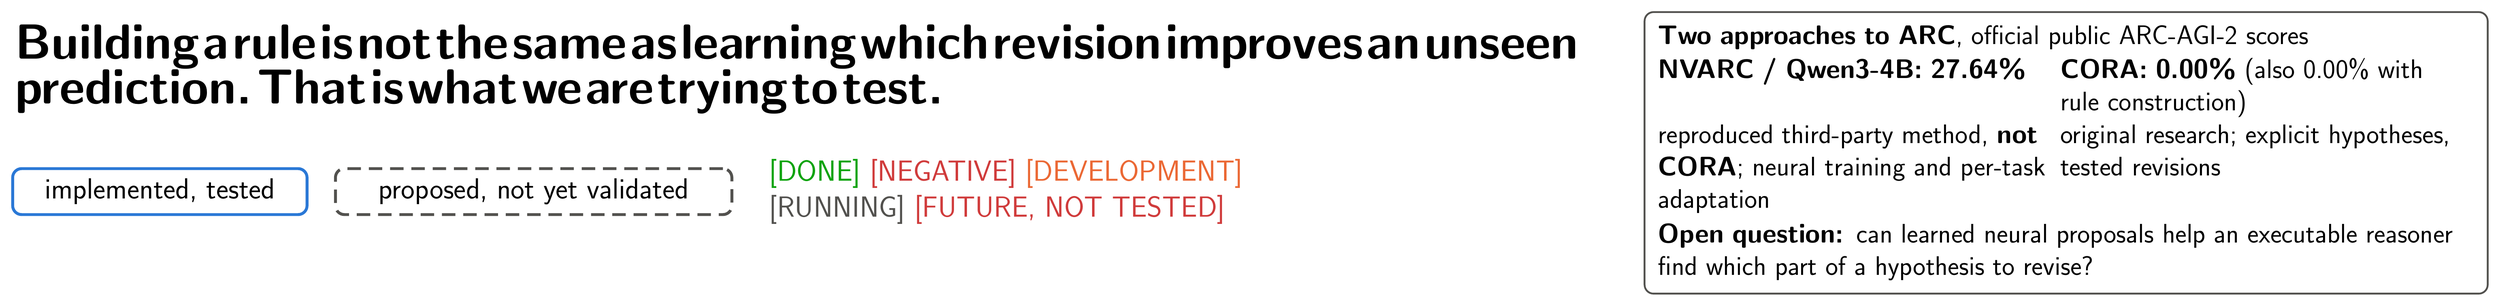
\begin{tikzpicture}
    \node[anchor=north west, text width=50cm, align=left] (bl) at (0,0) {\fontsize{44}{53}\selectfont\bfseries
      Building a rule is not the same as learning which revision improves an unseen prediction. That is what we are
      trying to test.};
    \node[stage, text width=8.6cm, anchor=north west] (s) at (0,-4.6) {implemented, tested};
    \node[pstage, text width=11.8cm, right=0.8cm of s] (d) {proposed, not yet validated};
    \node[right=1.0cm of d, font=\secfont, align=left] {{\color{good}[DONE]} {\color{critical}[NEGATIVE]}
      {\color{warm}[DEVELOPMENT]}\\ {\color{ink2}[RUNNING]} {\color{critical}[FUTURE, NOT TESTED]}};
    \node[anchor=north west, text width=25.6cm, align=left, draw=ink2, line width=1.6pt, rounded corners=8pt,
          inner sep=12pt, font=\fontsize{24}{29}\selectfont] (nb) at (51.2,0.3) {%
      \textbf{Two approaches to ARC}, official public ARC-AGI-2 scores\\[0.2em]
      \begin{tabular}{@{}>{\raggedright\arraybackslash}p{12.2cm}>{\raggedright\arraybackslash}p{12.6cm}@{}}
      \textbf{NVARC / Qwen3-4B: 27.64\%} & \textbf{CORA: 0.00\%} (also 0.00\% with rule construction)\\
      reproduced third-party method, \textbf{not CORA}; neural training and per-task adaptation &
      original research; explicit hypotheses, tested revisions\\
      \end{tabular}\\[0.2em]
      \textbf{Open question:} can learned neural proposals help an executable reasoner find which part of a hypothesis
      to revise?};
  \end{tikzpicture}
  \par\vspace{0.3em}
  {\fontsize{22}{27}\selectfont\color{ink2}
  Related work: Popper (Cropper \& Morel 2021); DreamCoder (Ellis et al.\ 2021); LILO (Grand et al.\ 2024); Model
  Discovery Agent (Murphy 2026). The failure-to-revision idea is not new; the question is which component to revise,
  against matched controls. Numbers: \texttt{records/CORA\_SUMMIT\_CLAIM\_LEDGER\_20261017.md} $\cdot$ AI coding
  assistance used for parts of the code and text $\cdot$ authorship pending collaborator review.\par}
}
\end{document}
